\documentclass{article}
\usepackage[utf8]{inputenc}
\usepackage[letterpaper, portrait, margin=1in]{geometry}
\usepackage{multicol}
\usepackage{amsmath}
\usepackage{amssymb}
\usepackage{enumerate}
\setlength\parindent{0pt}
\usepackage{enumerate}
\usepackage{graphicx}
\graphicspath{ {./images/} }
\usepackage{fancyhdr}
\usepackage{tcolorbox}
\usepackage{mathtools}
\newcommand{\sheader}[1]{\underline{#1:}}
\newcommand{\ftrans}{\xleftrightarrow[]{f}}
\newcommand{\ejw}{{e^\jomega}}


\newcommand{\header}[1]{\begin{large}\noindent #1\end{large}\\\rule{\textwidth}{0.5pt}}
\newcommand{\gap}{\medskip\\}
\newcommand{\centertext}[1]{\begin{center}#1\end{center}}
\newcommand{\bfrac}[2]{\left(\frac{#1}{#2}\right)}
\newcommand{\formula}[3]{\begin{center} \begin{tcolorbox}[title = #2] $$#3$$\end{tcolorbox}\end{center}}
\newcommand{\where}{\hspace{0.5cm} \textrm{where} \hspace{0.5cm}}
\newcommand{\hgap}{\hspace{0.5cm}}
\newcommand{\pfrac}[2]{\frac{\partial #1}{\partial #2}}
\newcommand{\jomega}{{j\omega}}
\newcommand{\domega}{d\omega}

\newcommand{\doubleformula}[4]{\begin{center} \begin{tcolorbox}[title = #2] $$#3$$\\$$#4$$\end{tcolorbox}\end{center}}

\newcommand{\tripleformula}[5]{\begin{center} \begin{tcolorbox}[title = #2] $$#3$$\\$$#4$$\\$$#5$$\end{tcolorbox}\end{center}}

\title{ELEC 221 Notes}
\author{reesecritchlow }
\date{September 2022}

\begin{document}

\begin{center}
    \Large ELEC 221 Notes\\
    \normalsize Reese Critchlow
\end{center}

\header{Notation}

\begin{align*}
    \textrm{Continuous Signals} && \textrm{Discrete Signals}\\
    x(t) && x(n)\\
    \textrm{Continuous-Time Systems} && \textrm{Discrete-Time Systems}\\
    x(t) \to y(t) && x[n] \to y[n]
\end{align*}
The arrow for systems means that for a given signal, say $x(t)$ when in putted into a system ($\to$) yields an output signal $y(t)$.
\\\gap
An equals sign ($=$) simply indicates equality between two signals.
\\\gap
\header{System Properties}
\begin{enumerate}
    \item \textbf{Memory}\\
    A system is \underline{memoryless} if the output at each time depends only on the input at the same time.\\
    Examples:
    \begin{align*}
        \textrm{Example: Voltage Through a Resistor} && V(t) = RI(t)\\
        \textrm {Counter Example: Voltage through a Capacitor} && V(t) = \frac{1}{C}\int_{-\infty}^tI(\tau)d\tau \\
        \textrm{Counter Example: A Delay System} && y[n] = x[n-1]
    \end{align*}
    Generally, a system where the function has some sort of time depenence which is not in the instantaneous current time period has a memory.
    
    \item \textbf{Invertibility}\\
    A system is \underline{invertible} if distinct inputs lead to distinct outputs.\\
    An example of a noninvertible system is $y(t) = x^2(t)$, because the square destroys a negative sign that may have existed in the input signal.
    
    \item \textbf{Causality}\\
    A system is \underline{causal} if the output at \textit{any time} depends only on the input at the present time or in the past. A comparison between causal systems and systems with memories may be able to be drawn, but they are not the same.
    \begin{multicols}{2}
        \underline{Causal Systems}
        \begin{itemize}
            \item Dependent events can only be in the present or in the past.
        \end{itemize}
        \vfill\null\columnbreak
        \underline{Memory-Bearing Systems}
        \begin{itemize}
            \item Dependent events can be in the present or in the future.
        \end{itemize}
        \vfill\null
    \end{multicols}
    A capacitor is causal, but a moving average, or time reversal is not.
    \item \textbf{Stability}\\
    A system is \underline{stable} if small changes in input do not cause the output to diverge.\\
    A stable system can also be described as one where bounded inputs lead to bounded outputs; essentially that the system never reaches an unbounded value.\\
    A system is also stable if \underline{the impulse response is absolutley integrable}.
    \item \textbf{Time Invariance}\\
    A system is \underline{time invariant} if time shifts in the input lead to identical time shifts in the output.\\
    \gap
    \underline{Proving Time Invariance}: Shift the input signal by a time period $a$, and pass it through the system. Shift the un-shifted output signal of the system by the same time period $a$. If they are the same signal, the system is time invariant.
    \item \textbf{Linearity}
    A \underline{linear} system has the following properties:
    
    \begin{center}
        \begin{multicols}{2}
            \underline{Additivity}
            \[
                x_1(t) + x_2(t) \to y_1(t) + y_2(t)
            \]
            \vfill\null\columnbreak
            \underline{Homogeneity}
            \[
                ax_1(t) \to ay_1(t)
            \]
            \vfill\null
        \end{multicols}
    \end{center}
    
    These two properties can also be combined:
    \[
        ax_1(t) + bx_2(t) \to ay_1(t) + by_2(t)
    \]
    
\end{enumerate}

\header{Harmonics}
A signal that has \textbf{only odd harmonics} requires that:
\[
    f\left(t+\frac{T}{2}\right) = -f(t)
\]
Whereas a signal that has \textbf{only even harmonics} requires that:
\[
    f\left(t + \frac{T}{2}\right) = f(t)
\]

\header{Impulse Response}

The \textbf{Impulse Response} of a system is the signal a system produces after a
unit impulse signal is passed through it. The unit impulse response is denoted by:
\begin{align*}
     h(n) && h[n].
\end{align*}
The impulse response is generally used to determine the ouput of a system 
by means of the convolution.
\gap
\header{Convolution}

The \textbf{Convolution} operation multiplies the entries of one signal by another in
a systematic fashion. It is defined by:
\begin{align*}
    x(t) \ast h(t) = \int_{-\infty}^\infty x(\tau) h(t- \tau) {d}\tau && x[n] \ast h[n] = \sum_{k=-\infty}^\infty x[k]h[n-k]    
\end{align*}
In this context, the convolution operator is being used to determine the output of a
signal through a system, given the system's impulse response.
\gap
\underline{Properties of the Convolution:} The convolution is:
\begin{itemize}
    \item Associative: $x \ast (y \ast z) = (x \ast y) \ast z$
    \item Commutative: $x \ast y = y \ast x$
    \item Distributive: $x \ast (y + z) = x \ast y + x \ast z$
\end{itemize}

\pagebreak

\header{Fourier Series (Continuous Time)}

Given a correct periodic signal, one can describe it as a sum of complex exponentials,
called a \textbf{Fourier Series}. 
\gap
Signals that can be expressed as a fourier series must obey the \underline{Dirichlet Conditions}:
\gap
If over one period, a signal $x(t)$:
\begin{enumerate}
    \item Is single-valued
    \item Is absolutley integrable
    \item Has a finite number of maxima and minima
    \item Has a finite number of discontinuities
\end{enumerate}
The Dirichlet conditions are sufficient but \underline{not necessary}, however. This
being said, they can tell us that the Fourier series \underline{converges} to:
\begin{itemize}
    \item $x(t)$ where it is continuous
    \item half the value of the jump if it is discontinuous.
\end{itemize}


The Fourier Series has two parts to it:
\begin{multicols}{2}
    \centertext{\underline{Fourier Synthesis Equation}}
    \[
        x(t) = \sum_{k = -\infty}^\infty c_k e^{jk\omega t}    
    \]
    \centertext{where $\omega$ is the fundamental frequency of the function.}
    \vfill\null\columnbreak
    \centertext{\underline{Fourier Analysis Equation}}
    \[
        c_k = \frac{1}{T}\int_T e^{-jk\omega t}x(t){d}t    
    \]
    \centertext{where $T$ is the period of the function.}
    \vfill\null
\end{multicols}

\underline{Gibbs Phenomena:} If a function represented by a Fourier series has discontinuities,
there will be ``imperfections'' or ``ringings'' in the Fourier series. This is known
as the Gibbs Phenomena, where it is known that there will be ``spikes'' of about $9\%$
the height of the discontinuity around the bounds of the discontinuity itself.
\gap
\header{Operations on Fourier Series}

\underline{Summation of Signals}
\smallskip\\
Given two signals with the same period:
\begin{align*}
    x_1(t) = \sum_{k = -\infty}^\infty c_{k(1)}e^{jk\omega t} && x_2(t) = \sum_{k = -\infty}^\infty c_{k(2)}e^{jk\omega t}
\end{align*}
Then we can find their sum as:
\begin{align*}
    y(t) = Ax_1(t) + Bx_2(t) = \sum_{k = -\infty}^\infty c_k e^{jk\omega t} && c_k = Ac_{k(1)} + Bc_{k(2)}
\end{align*}
\underline{Time Shifting}
\smallskip\\
Given a signal, its timeshift, $x(t) \to x(t - t_0)$ can be obtained by:
\begin{align*}
    x(t - t_0) = \sum_{k = -\infty}^\infty c'_k e^{jk\omega t} && c'_k = e^{-jk\omega t_0}\cdot c_k
\end{align*}
\underline{Convolution of Signals}
Given two signals with the same fundamental frequency*:
\begin{align*}
    x_1(t) = \sum_{k = -\infty}^\infty c_{k(1)}e^{jk\omega t} && x_2(t) = \sum_{k = -\infty}^\infty c_{k(2)}e^{jk\omega t}
\end{align*}
Then the convolution of the signals takes the form of:
\begin{align*}
    y(t) = x_1(t) \ast x_2(t) = \sum_{k = -\infty}^\infty c_k' e^{jk\omega t} && c'_k = \sum_{l = -\infty}^\infty a_l b_{k - l}
\end{align*}
\gap
\header{Signal Power and Energy}

We can define the power and energy of a periodic function over a single period. 
\begin{multicols}{2}
    \centertext{\underline{Energy of a Signal}}
    \[
        E = \int_T \left|x(t)\right|^2 dt    
    \]
    \vfill\null\columnbreak
    \centertext{\underline{Power of a Signal}}
    \[
        P = \frac{1}{T}\int_T \left|x(t)\right|^2 dt    
    \]
    \vfill\null
\end{multicols}

Power and energy can also be used to show \underline{Parseval's Relation}.

\[
    \frac{1}{T}\int_T\left|x(t)\right|^2 dt = \sum_{k = -\infty}^\infty |c_k|^2    
\]

\header{Discrete Time Fourier Series}
\underline{Precursor -- Differences between DT and CT periodic signals}: There are 
two main differences between DT and CT periodic signals. 
\begin{enumerate}
    \item Frequency does not increase infinitley with $\omega$.
    \smallskip\\
    For some $x[n]$ with period T:
    \begin{align*}
        x[n] &= e^{\frac{2\pi n}{T}j}\\
        &= e^{\frac{2\pi (n + N)}{T}j}\\
        &= e^{\frac{2\pi n}{T}j}e^{\frac{2\pi N}{T}j}\\
        & \textrm{But if } N > T,\\
        &= e^{\frac{2\pi n}{T}j}e^{\frac{2\pi (T\alpha + N')}{T}j}\\
        &= e^{\frac{2\pi n}{T}j}e^{\frac{2\pi (N')}{T}j}e^{{2\pi \alpha}j}\\
        &= e^{\frac{2\pi n}{T}j}e^{{2\pi (N')}}
    \end{align*}
    It is important to note that this same result does not hold in CT because the
    resolution of $\alpha$ is not restricted to $\mathbb{Z}$.
    \item $\frac{\omega}{2\pi}$ must be rational for the signal to be periodic.
    \gap
    \underline{Note:} If $\frac{\omega}{2\pi}$ is a fraction, the numerator is the period.
\end{enumerate}
Now, we can define the Fourier synthesis and analysis equations for discrete time.
\begin{multicols}{2}
    \centertext{\underline{Fourier Synthesis Equation}}
    \[
        x[n] = \sum_{k = 0}^{N - 1}c_k e^{jk \frac{2\pi n}{N}}   
    \]
    \centertext{where $N$ is the period or number of samples of the function.}
    \vfill\null\columnbreak
    \centertext{\underline{Fourier Analysis Equation}}
    \[
        c_k = \frac{1}{N}\sum_{n = 0}^{N - 1}x[n]e^{-jk \frac{2\pi n}{N}}   
    \]
    \centertext{where $N$ is the period or number of samples of the function.}
    \vfill\null
\end{multicols}

\header{The Frequency Response}

The \textbf{Frequency Response} or the \textbf{System Response} of a system, denoted
by $H(j\omega)$ describes how frequencies are attenuated, amplified, and phase shifted
in a system. 
\smallskip\\
It is computed by:
\begin{align*}
    H(j\omega) = \int_{-\infty}^\infty e^{j\omega \tau}h(\tau){d}\tau 
\end{align*}
\underline{Question:} Are there frequency responses in DT?
\gap
\underline{Using the Frequency Response:} To use the frequency response, to compute
how a system changes a signal, there are three steps.
\begin{enumerate}
    \item Compute the frequency response (if it isn't already given).
    \item Compute the Fourier coefficients of the signal.
    \item Apply the frequency response to each of the Fourier coefficents to obtain
    the output signal.
\end{enumerate}
This can be generalized to:
\begin{align*}
    x(t) \to y(t) = \sum_{k = -\infty}^\infty c_k H(jk \omega)e^{jk\omega t} &&
    x[n] \to y[n] = \sum_{k = 0}^{N - 1}c_k H(e^{jk\omega})e^{jk\omega n}
\end{align*}

\header{Filters}
We can characterize filters by their frequency responses, $H$.
\gap
\underline{Filters in Discrete Time:} It is important to note that a filter in DT
is mirrored across zero. Frequencies increase up until $\omega = \pi$ and then
subsequently decrease.
\gap
\underline{Categories of Filters:} Filters can be broken up into two main categories:
\begin{enumerate}
    \item Infinite Impulse Response (IIR)\\
    Infinite impulse response filters are those whose impulse response \underline{does not}
    become zero over a finite amount of time.
    \item Finite Impulse Response (FIR)\\
    Finite impulse response filters are thos whose impulse response \underline{does} 
    become zero over a finite amount of time.
\end{enumerate}

\pagebreak

\header{The Fourier Transform}
The \textbf{Fourier Transform}, not to be confused with the \textit{Fourier series}
employs the principles of the \textit{Fourier series} to \underline{aperiodic signals}.
Thus, the equations governing it are:

\begin{multicols}{2}
    \centertext{\underline{Inverse Fourier Transform}}
    \[
        x(t) = \frac{1}{2\pi}\int_{-\infty}^\infty X(j\omega)e^{j\omega t}{d}\omega
    \]
    \vfill\null\columnbreak
    \centertext{\underline{Fourier Transform (Fourier Spectrum)}}
    \[
        X(\jomega) = \int_{-\infty}^\infty x(t)e^{-\jomega t}{d}t  
    \]
    \vfill\null
\end{multicols}
A more physical intuition of the Fourier transform is that it takes
a signal and decomposes it into a spectrum of its frequencies. This
is called the \underline{Fourier Spectrum}.
\gap
\underline{Fourier Transform and Impulse Response:} The Fourier
transform can be used to obtain the frequency response from the impulse response
and vice versa. This forwards direction of this was already known however.

\begin{multicols}{2}
    \centertext{\underline{Continuous Time}}
    \begin{align*}
        h[n] &= \frac{1}{2\pi}\int_{2\pi}H(e^\jomega)e^{\jomega n} \domega\\
        H(\jomega) &= \int_{-\infty}^\infty e^{-\jomega \tau}h(\tau)d\tau
    \end{align*}
    \vfill\null\columnbreak
    \centertext{\underline{Discrete Time}}
    \begin{align*}
        h(t) &= \frac{1}{2\pi}\int_{-\infty}^\infty e^{j\omega t}H(\jomega)\domega \\ 
        H(e^{\jomega}) &= \sum_{n = -\infty}^\infty e^{-\jomega n }h[n]
    \end{align*}
    \vfill\null
\end{multicols}

\pagebreak

\section*{Midterm 2}

\header{Properties of Fourier Transforms}

\sheader{Multiplication Property} We can shift the frequency spectrum of a signal by using the \underline{multiplication property}.
This comes in the form:
\begin{align*}
    x(t) \cdot e^{j\omega_c t} \xleftrightarrow[]{f}  X(j(\omega - \omega_0))
\end{align*}

\sheader{Differentiation} Differentiation also is made easy under 
Fourier transforms.

\begin{align*}
    \frac{dx(t)}{dt} \ftrans \jomega X(jw)
\end{align*}

\sheader{Integration}

\begin{align*}
    \int_{-\infty}^t x(\tau) d\tau \ftrans \frac{1}{\jomega}X(\jomega) + \pi X(0)\delta(\omega)
\end{align*}

We can also chain all of these together with successive multiplications
in the frequency domain.
\gap
\sheader{Differential Equations under Fourier Transforms} One can obtain
the transfer function of a differential equation under a fourier transform.
Given a differential equation of the form:
\begin{align*}
    \sum_{k = 0}^N \alpha_k \frac{d^ky(t)}{dt^k} = \sum_{k = 0}^M \beta_k \frac{d^k x(t)}{dt^k}
\end{align*}
We can obtain its transfer function:
\begin{align*}
    H(j\omega) = \frac{Y(\jomega)}{X(\jomega)} = \frac{\sum_{k = 0}^M \beta_k (\jomega)^k}{\sum_{k = 0}^N\alpha_k(\jomega)^k}
\end{align*}
This formula is kind of confusing. It's important to just note it as:
\begin{align*}
    H(\jomega) = \frac{\sum x\textrm{ coeffs}\cdot (\jomega)^k}{\sum y \textrm{ coeffs} \cdot (\jomega)^k}
\end{align*}
\sheader{Difference Equations under Fourier Transforms} 
We can also apply the same formulae to difference equations:
\begin{align*}
    \sum_{k = 0}^N \alpha_k y[n - k] = \sum_{k = 0}^M \beta_k x[n - k]
\end{align*}
Thus, resulting in a similar formula:
\begin{align*}
    H(e^\jomega) = \frac{Y(\jomega)}{X(\jomega)} = \frac{\sum_{k = 0}^M \beta_k e^{-jk\omega}}{\sum_{k = 0}^M \alpha_k e^{-jk\omega}} = \frac{\sum x \textrm{ coeffs} \cdot e^{-jk\omega}}{\sum y \textrm{ coeffs} \cdot e^{-jk\omega}}
\end{align*}

\pagebreak

\header{The Discrete Time Fourier Transform}

The \underline{Discrete Time Fourier Transform} is used for transforming
\textbf{discrete, aperiodic signals}. It is as follows:
\begin{multicols}{2}
    \centertext{\underline{Inverse DTFT (Synthesis)}}
    \begin{align*}
        x[n] = \frac{1}{2\pi}\int_{2\pi}X(e^\jomega)e^{\jomega n}d\omega
    \end{align*}
    \vfill\null\columnbreak
    \centertext{\underline{DTFT (Analysis)}}
    \begin{align*}
        X(e^\jomega) = \sum_{n = -\infty}^\infty x[n] e^{-j\omega n}
    \end{align*}
    \vfill\null
    
\end{multicols}

We also require \underline{convergence criteria} in the DTFT. It is as follows:
\begin{align*}
    \sum_{n=-\infty}^\infty | x[n] | < \infty && \sum_{n = -\infty}^\infty |x[n]|^2 < \infty
\end{align*}
Only \underline{one} of these criteria must be satisfied.
\gap
There exist the same properites for the CT Fourier transform, however, some more
properties aries in the DTFT:
\gap
\sheader{Conjugation} 

\begin{align*}
    \textrm{Even}(x[n]) \ftrans \textrm{Re}(X(\ejw)) && \textrm{Odd}(x[n]) \ftrans j\cdot \textrm{Im}(X(\ejw))
\end{align*}

\sheader{Periodicity}
\begin{align*}
    X(e^{j(\omega + 2\pi)} = X(\ejw))
\end{align*}

\sheader{Differentiation in Frequency} (Warning: this is \underline{very} different.)
\begin{align*}
    n \cdot x[n] \ftrans j \frac{d X(\ejw)}{d\omega}
\end{align*}

\sheader{Differencing}
\begin{align*}
    x[n] - x[n - 1] \ftrans (1 - e^{-\jomega} )X(\ejw)
\end{align*}

\sheader{Accumulating}
\begin{align*}
    \sum_{m = -\infty}^n x[m] \ftrans  \frac{1}{1 - e^{-\jomega}}X(\ejw) + \pi X(e^{j0})\sum_{k = -\infty}^\infty \delta(w - 2\pi k)
\end{align*}

\sheader{Parseval's Theorem} We can also define Parseval's theorem in the DTFT.
\begin{align*}
    \sum_{n = -\infty}^\infty |x[n]|^2 = \frac{1}{2\pi} |X(\ejw)|^2 d\omega
\end{align*}

\header{The Fast Fourier Transform}

It's cool. It has $N\log_2{N}$ time complexity.

\pagebreak

\header{Frequency Responses of LTI Systems}

We can look at the frequency responses of LTI systems with a slightly different prespective.
\gap
Since a transfer function, $H(\jomega)$ or $H(\ejw)$ has both a magnitude and a phase,
we can write a transfer function, or any frequency spectrum as:
\begin{align*}
    H(\jomega) = |H(\jomega)| e^{\angle H(\jomega)}
\end{align*}

Hence, we can write input and ouptut signals as follows:
\begin{align*}
    |Y(\jomega)| &= |H(\jomega)||X(\jomega)| \\
    \angle Y(\jomega) &= \angle H(\jomega) + \angle X(\jomega)
\end{align*}

\sheader{Group Delay} We can also define how much a system delays its input signal
through the \underline{group delay}. 
\begin{align*}
    \tau(\omega) = -\frac{d}{d\omega} \left(\angle H(\jomega)\right)
\end{align*}

\header{Step Response}

Under an ideal filter, a step function attains some sort of ``ringing'' in the
graph. Thus, we find it important to define the \underline{step response}
for systems.
\gap
Computing the step response is as follows:
\begin{align*}
    s(t) = \int_{-\infty}^t h(\tau) d\tau
\end{align*}

\header{Bode Plots}

Often, we find ourselves in situations where plotting phase and magnitudes of transfer
functions is difficult because of multiplication/division. Thus, we can use a 
\underline{Bode Plot}. The process for obtaining a Bode Plot is as follows:

\begin{multicols}{2}
    \centertext{\underline{Magnitude}}
    \begin{enumerate}
        \item Take $-20\log_{10}|H(\jomega)|$
        \item Identify the point(s), $\tau_n$ for which the function has an 
        ``inflection point''.
        \item Take $\omega \gg \tau_n$ and $\omega \ll \tau_n$, and plot 
        the two behaviours.
    \end{enumerate}
    \vfill\null\columnbreak
    \centertext{\underline{Phase}}
    \begin{enumerate}
        \item Plot against $\log_{10}\omega$.
    \end{enumerate}
\end{multicols}

\pagebreak

\header{Sampling Theory}
Given a signal $x(t)$, we can define an ``impulse train'' $p(t)$, which is a train
of impulses that ``sample'' our signal at a given interval $T$. We can also
define our \underline{sampling frequency} to be:
\begin{align*}
    \omega_s = \frac{2\pi}{T}.
\end{align*}

Hence, we can define our \underline{sampled signal} $x_p(t) = x(t) \cdot p(t)$.
\begin{align*}
    x_p(t) = \sum_{n = - \infty}^\infty x(nT) \cdot \delta(t - nT).
\end{align*} 

Given a sampled signal, it is natural to investigate the frequency spectrum of 
$x(t)$, $p(t)$, and $x_p(t)$. Hence, we can derive the Fourier transforms for each:
\begin{multicols}{3}
    \centertext{\underline{$X(\jomega)$}}
    \begin{align*}
        X(\jomega) = X(\jomega)
    \end{align*}
    \vfill\null\columnbreak
    \centertext{\underline{$P(\jomega)$}}
    \begin{align*}
        P(\jomega) = \frac{2\pi}{T}\sum_{k = \infty}^\infty \delta(\omega - k\omega_s)
    \end{align*}
    \vfill\null\columnbreak
    \centertext{\underline{$X_p(\jomega)$}}
    \begin{align*}
        X_p(\jomega) = \frac{1}{T} \sum_{k = -\infty}^\infty X(j(\omega - k\omega_s))
    \end{align*}
    \vfill\null
\end{multicols}

It's also very important to get a grasp on the graphs that result from these functions:
\\
\begin{center}
    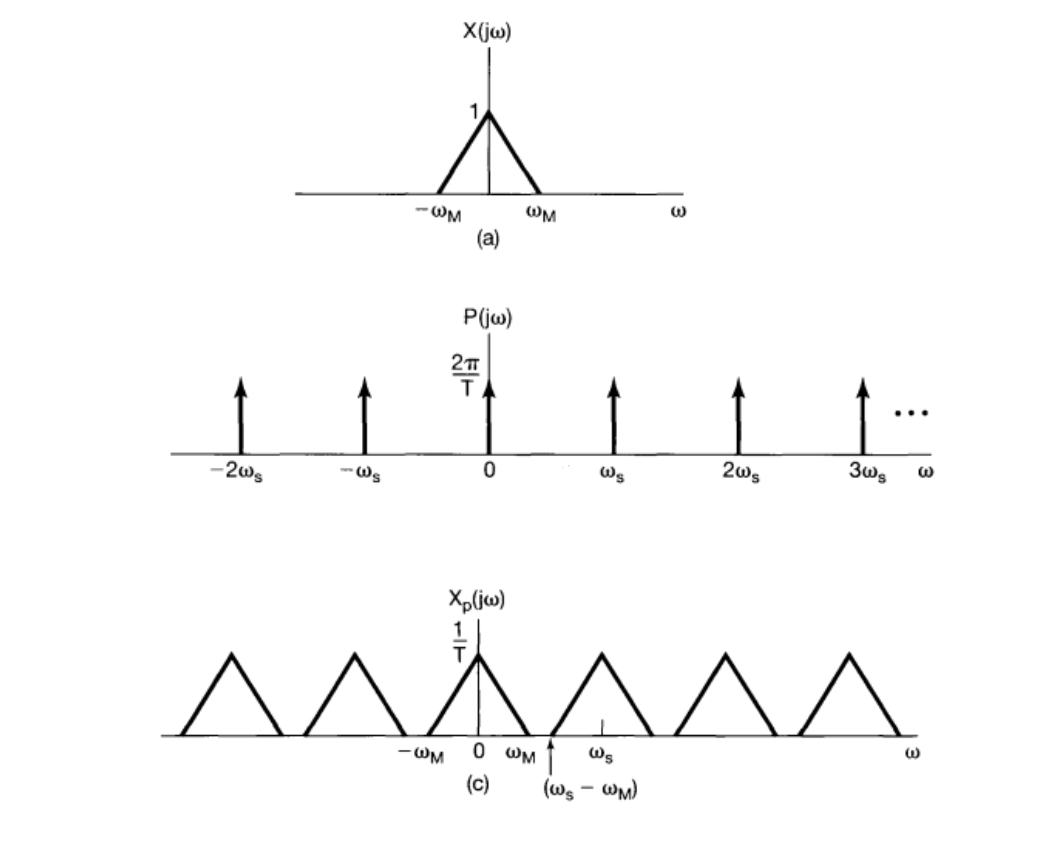
\includegraphics[scale=0.45]{sampling-graphs.png}    
\end{center}
Note that for the graph of $X_p(j\omega)$ has the $\omega_s - \omega_m$, which will
be important later. $\omega_m$ is defined as the maximum frequency contained in the
input signal.
\gap
Hence, the question may be posed: How can retrieve the original signal from the
sampled signal? The answer to this question is the \textbf{Sampling Theorem}:
\gap
\sheader{Sampling Theorem (condensed)}
Any signal can be reconstructed if the sampling frequency is \textit{strictly} larger than twice
the maximum frequency in the sampled signal. In math, this looks like:
\begin{align*}
    \omega_s > 2\omega_m
\end{align*} 
Hence, we can also define:
\begin{itemize}
    \item \sheader{Nyquist Rate} $\omega_s = 2\omega_M$
    \item \sheader{Nyquist Frequency} $\omega_M = \omega_s / 2$
\end{itemize}

\pagebreak

\header{Interpolation}
Often, we cannot always fully reconstruct our signal from the sampled signal, due
to a sampling rate that is too low. Hence, there are some methods in which 
we can \textit{interpolate} the sampled signal to attempt to reconstruct the 
original signal. Some of these methods include, but are not limited to:
\begin{itemize}
    \item \sheader{Zero Order Hold} Assume each point maintains the same value
    until the next sample is available.
    \item \sheader{Band Limited Interpolation} Apply a lowpass filter to the 
    system, with cutoff $\omega_c$ and gain $T$.
    \begin{align*}
        x_r(t) = \sum_{n = \infty}^\infty x(nT)\frac{\omega_c T \sin(\omega_c(t - nT))}{\pi \omega_c(t - nT)}
    \end{align*}
\end{itemize}

\header{Aliasing}

An important phenomena arises when you don't sample at a high enough rate: \textbf{aliasing}.
\gap
Essentially, the frequencies in $X_p(\jomega)$ begin to overlap, and the frequency
spectrum of the original spectrum becomes distorted.
\gap
\header{Conversions Between DT and CT}

Many common computing practices see the conversion of a signal from CT to DT and then
back to CT in order to employ computational methods of signal processing. For such
a process, we define a standard process for such signal processing.

\begin{enumerate}
    \item Original signal $x_c(t)$ is sampled by an impulse train $p(t)$ to form
    the sampled signal $x_p(t)$.
    \item Sampled signal is converted to a discrete time signal $x_d[n]$.
    \item Discrete signal is processed through $H_d(\ejw)$.
    \item Processed, discrete signal is transformed back into a CT signal.
    \item CT signal is low-passed to recover the original signal.
\end{enumerate}

Hence, when converting to a DT signal, we find ourselves with a new frequency 
defining our Fourier spectrum, $\Omega$.
\gap
Thus, the Fourier spectrum for the transformed signal ends up being defined as:
\begin{align*}
    X_d(\ejw) = X_p(j\Omega / T)
\end{align*}
Thus, we can also define the new frequency, $\Omega$.
\begin{align*}
    \Omega = \omega T.
\end{align*}
It's also important to define the signal in discrete time:
\begin{align*}
    x_c[n] = x_c(nT)
\end{align*}

\header{Decimation/Downsampling}
Downsampling occurs when samples are removed from a DT signal in a process as such:
\begin{align*}
    x_p[n] = \begin{cases}
        x[n] & N \mid \textrm{n}\\
        0 & \textrm{otherwise}
    \end{cases}
\end{align*}
Where $N$ describes every $N$th sample to take. 
\gap
In the case of downsampling, we find that the frequency spectrum is altered.
\begin{align*}
    X_b(\ejw) = X_p(e^{\frac{\jomega}{N}})
\end{align*}
Upsampling also exists:
\begin{align*}
    X_u(\ejw) = X_p(e^{\jomega N})
\end{align*}

\pagebreak

\section*{Final Exam}

\header{Amplitude Modulation}

To send and recieve signals, a technique called \underline{amplitude modulation} is often 
utilized. The main principle behinde amplitude modulation is that a band-limited frequency
can be frequency-shifted up such that multiple different signals can be broadcasted on the 
same summed signal. Hence, for this technique, there generally is a ``carrier signal''
which is responsible for the modulation of frequency. Generally, these carrier signals 
(in this course) come in two forms:
\begin{itemize}
    \item \sheader{Complex Exponential Signals} $\displaystyle c(t) = e^{j(\omega_c t + \theta_c)}$
    \item \sheader{Sinusoidal Signals} $\displaystyle c(t) = \cos(\omega_c t + \theta_c)$
\end{itemize}
The original signal is then multiplied with the carrier signal $x(t)c(t)$, since 
multiplication in the time domain implies convolution in the frequency domain.
\gap
\sheader{Amplitude Modulation using Complex Exponentials} Amplutde modulation using 
complex exponentials is relativley straightfoward. Since the amplitude is preserved,
then the frequency is only shifted up by $\omega_c$. Hence, we can outline a process:
\begin{enumerate}
    \item Original signal $x(t)$ is multiplied by the carrier signal $c(t) = e^{\jomega_c t}$, $y(t) = x(t)c(t)$.
    The frequency domain of $y(t)$ is then simply the original signal shifted up by $\omega_c$.
    \item Signal is broadcasted.
    \item Signal is demodulated using a similar carrier signal $c'(t) = e^{-\jomega_c t}$, $x(t) = c'(t)y(t)$.
    \item The original signal is recovered.
\end{enumerate}

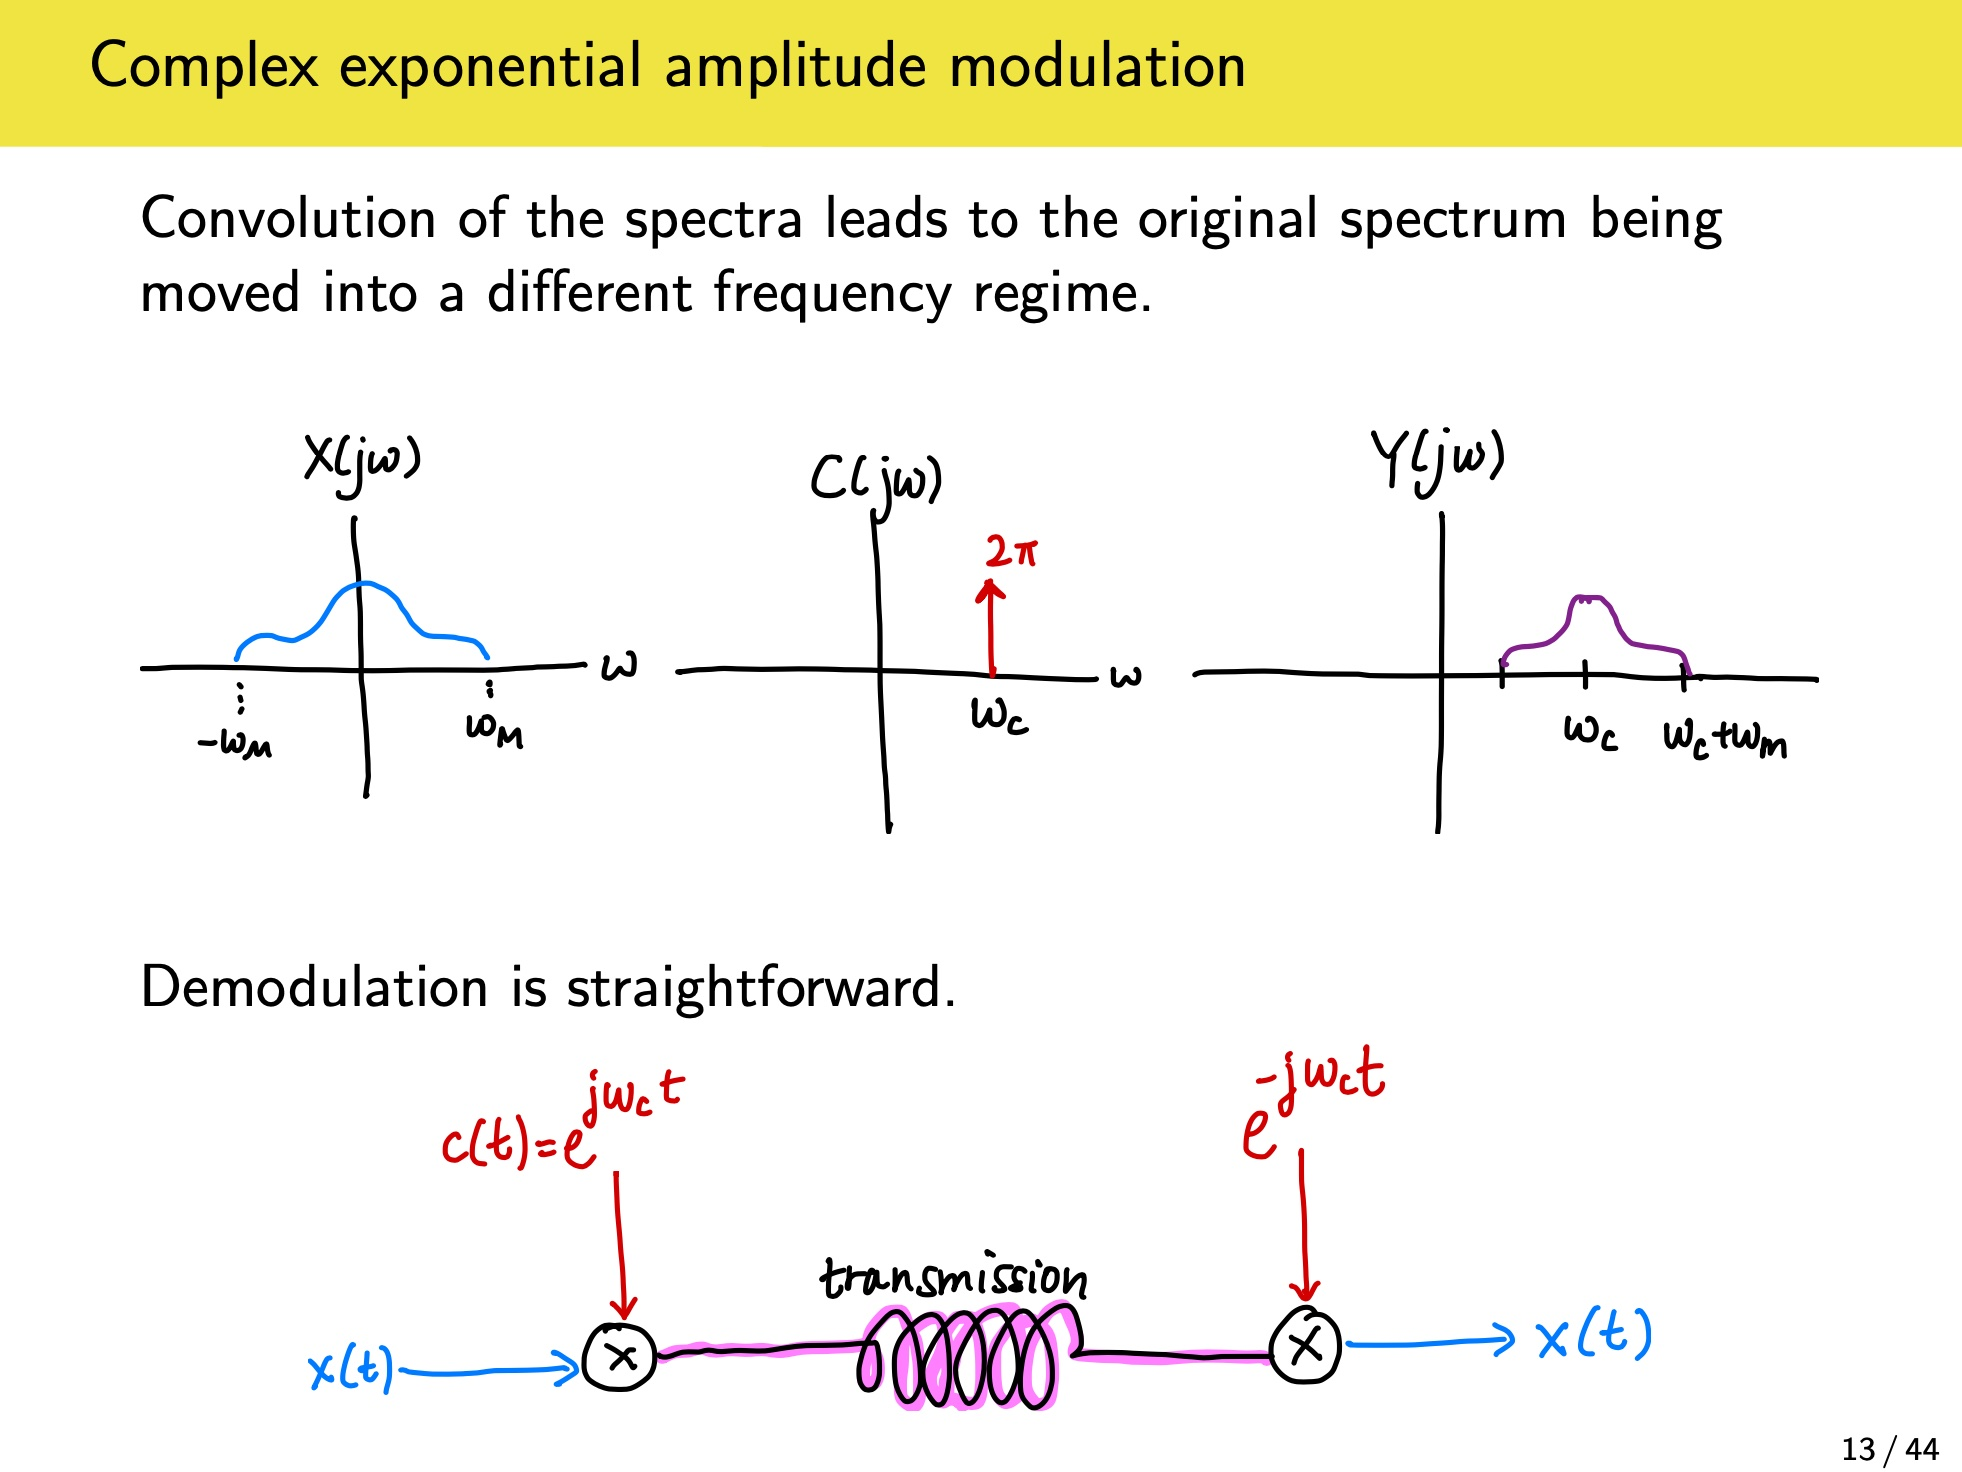
\includegraphics[scale=0.13]{exponential-modulation.jpg}

\sheader{Amplitude Modulation using Sinusoids} When using sinusoids, there exist some 
more uances. Since the frequency spectrum of a sinusoid has both a positive and 
a negative part, then two signals are outputs of the convolution of the carrier signal 
and the original signal. It also is more challenging since a the frequency spectrum of a 
sinusoid is also scaled down by $\frac{1}{2}$. Hence, when demodulating the signal,
we require that it is subsequently band-pass filtered and applied a gain of 2.

\begin{enumerate}
    \item Original signal $x(t)$ is multiplied by the carrier signal $c(t) = \cos(\omega_c t)$ $y(t) = x(t)c(t)$.
    \item 
\end{enumerate}


\end{document}